\documentclass{article}
\usepackage[sexy, hdr, fancy]{evan}
\usepackage{listings}
\usepackage{graphicx}
\graphicspath{.}
\lstset{language=Matlab}
\setlength{\droptitle}{-4em}

\lhead{Homework 1 Solutions}
\rhead{Linear Algebra and Differential Equations}
\lfoot{}
\cfoot{\thepage}

\begin{document}
\title{Homework 1 Solutions}
\maketitle
\thispagestyle{fancy}

\begin{enumerate}
	\item Show that the following ODE is exact and solve it.
		\begin{align*}
			(\sin y + y\cos x)\, dx + (\sin x + x\cos y)\, dy = 0 \quad y(2)=3
		\end{align*}
		\begin{soln}
			This equation is in the form
			\begin{align*}
				M(x, y)\, dx + N(x, y)\, dy = 0
			\end{align*}
			where
			\begin{align*}
				M(x, y) &= \sin y + y\cos x \\ 
				N(x, y) &= \sin x + x\cos y
			\end{align*}
			Now, the partial derivatives of $M$ and $N$ are
			\begin{align*}
				\frac{\partial M}{\partial y} &= \cos y + \cos x \\
				\frac{\partial N}{\partial x} &= \cos x + \cos y
			\end{align*}
			Since these two partials are equal, the ODE is exact. 

			To solve this ODE, we can either use Eq (29), or use the process outlined in the proof of Theorem 1. If $F(x, y)$ is the general solution, then we have
			\begin{align*}
				F(x, y) &= \int M(x, y)\, dx + g(y) = \int (\sin y + y\cos x)\, dx + g(y) \\
				&= x\sin y + y\sin x + g(y)
			\end{align*}
			We also have the condition $\partial F/\partial y = N(x, y),$ which means
			\begin{align*}
				\frac{\partial}{\partial y} \left[ x\sin y + y\sin x + g(y) \right] &= x\cos y + \sin x + g'(y) \\
				&= \sin x + x\cos y \\ 
				\implies g(y) &= C_1 \\
				\implies F(x, y) &= x\sin y + y\sin x + C_1
			\end{align*}
			so the general solution of the ODE is given implicitly by the equation
			\begin{align*}
				x\sin y + y\sin x = C
			\end{align*}
			Since we are given the initial value $y(2)=3,$ we know the point $(2, 3)$ lies on the solution, so substituting this into the general solution, we have
			\begin{align*}
				2\sin 3 + 3\sin 2 = C
			\end{align*}
			and thus the particular solution is 
			\begin{align*}
				\boxed{x\sin y + y\sin x = 2\sin 3 + 3\sin 2}
			\end{align*}
		\end{soln}

		\newpage
	\item Find a suitable integrating factor, if possible, and use it to find a general solution of the following ODE.
		\begin{align*}
			(\cos y)\, dx = \left[ 2(x-y)\sin y + \cos y \right]\, dy
		\end{align*}
		NOTE: $\cos 2\theta = 2\cos^2\theta-1.$
		\begin{soln}
			Moving everything to one side, this differential equation is
			\begin{align*}
				\cos y\, dx + \left[ 2(y-x)\sin y - \cos y \right]\, dy &= 0
			\end{align*}
			Here,
			\begin{align*}
				M(x, y) &= \cos y \implies M_y = -\sin y \\
				N(x, y) &= 2(y-x)\sin y - \cos y \implies N_x = -2\sin y
			\end{align*}
			so the equation is not exact as written, but we notice that
			\begin{align*}
				\frac{N_x-M_y}{M} = \frac{-2\sin y -(-\sin y)}{\cos y} = -\tan y
			\end{align*}
			is a function of just $y,$ so we can multiply by the integrating factor
			\begin{align*}
				\exp\left( \int -\tan y\, dy \right) = \exp\left( \ln \cos\abs{y} \right) = \cos y
			\end{align*}
			which gives the equation
			\begin{align*}
				\cos^2 y \, dx + \left[ 2(y-x)\sin y\cos y - \cos ^2 y \right]\, dy &= M_1(x, y)\, dx + N_1(x, y)\, dy = 0
			\end{align*}
			Now, the equation is exact, so to solve for the solution, we integrate to solve for $F:$
			\begin{align*}
				F(x, y) &= \int M_1(x, y)\, dy = \int \cos^2y\, dx = x\cos^2y + g(y)
			\end{align*}
			We also have the condition $\frac{\partial}{\partial y} F(x, y) = N_1(x, y),$ so
			\begin{align*}
				\frac{\partial}{\partial y} \left[ x\cos^2 y + g(y) \right] &= -2x\sin y\cos y + g'(y) = N_1(x, y) \\
				&= 2y\sin y\cos y - 2x\sin y \cos y - \cos^2 y \\
				\implies g'(y) &= 2y\sin y\cos y - \cos^2 y \\
				&= y\sin 2y - \frac{1}{2}(\cos 2y + 1) \\
				\implies g(y) &= \int \left[ y\sin 2y - \frac{1}{2}(\cos 2y + 1) \right]\, dy \\
				&= \int y\sin 2y\, dy - \int \frac{1}{2}\cos 2y\, dy - \int \frac{1}{2}\, dy \\
				&= -\frac{y}{2}\cos 2y - \int \left( -\frac{1}{2}\cos 2y \right)\, dy - \int \frac{1}{2}\cos 2y\, dy - \frac{y}{2} \\
				&= -y\left( \frac{\cos 2y + 1}{2} \right) = -y\cos^2 y
			\end{align*}
			Where we integrated $g(y)$ using integration by parts. Thus the general solution is given implicitly by
			\begin{align*}
				F(x, y) = x\cos^2y -y\cos^2y = \boxed{(x-y)\cos^2y = C} \\
			\end{align*}

			As an alternative solution, this ODE is equivalent to
			\begin{align*}
				\frac{dx}{dy} &= \frac{2(x-y)\sin y + \cos y}{\cos y} = 2x\tan y - 2y\tan y + 1 \\
				\implies \frac{dx}{dy} + (-2\tan y) x &= -2y\tan y + 1
			\end{align*}
			This is a linear first-order differential equation in $x$ with $P(y)=-2\tan y$ and $Q(y) = -2y\tan y + 1.$ Thus, the integrating factor is
			\begin{align*}
				p(y) &= \exp\left( \int P(y)\, dy \right) = \exp\left( \int -2\tan y\, dy \right) \\ 
				&= \exp\left( 2\ln\abs{\cos y} \right)= \cos^2 y
			\end{align*}
			Thus we have
			\begin{align*}
				\cos^2 y \left( \frac{dx}{dt} -2x\tan y \right) &= \cos^2y \left( -2y\tan y+ 1 \right) = \cos^2y \left( -2y\cdot \frac{\sin y}{\cos y} + 1 \right) \\
				&= -2y\sin y\cos y + \cos^2y \\
			\end{align*}
			Now, using the trig identities $\sin 2y = 2\sin y\cos y$ and
			\begin{align*}
				\cos 2y = 2\cos^2y - 1 \implies \cos^2y = \frac{1}{2} + \frac{1}{2}\cos 2y
			\end{align*}
			we can integrate the left and right sides of the ODE modified with the integrating factor to get
			\begin{align*}
				x(y) \cos^2y &= \int\left( -y\sin 2y + \frac{1}{2} + \frac{1}{2}\cos 2y \right)\, dy = \int\left( -y\sin 2y \right)\, dy + \int \frac{1}{2}\, dy + \int \frac{1}{2}\cos 2y\, dy
			\end{align*}
			The first integral can be evaluated using integration by parts using $u=y$ and $dv=-\sin 2y,$ so we get 
			\begin{align*}
				x(y)\cos^2 y &= \frac{y}{2}\cos 2y - \int \frac{1}{2}\cos 2y\, dy + \int\frac{1}{2}\, dy + \int\frac{1}{2}\cos 2y\, dy \\
				&= \frac{y}{2}\cos 2y + \frac{y}{2}  + C = \frac{y}{2}\left( \cos 2y + 1 \right) + C \\
				&= \frac{y}{2}\left( 2\cos^2y-1+1 \right) + C = y\cos^2y + C \\
				\implies x(y) &= \boxed{y + \frac{C}{\cos^2 y}}
			\end{align*}
			is the general solution to the ODE, which agrees with the first solution.

		\end{soln}

		\newpage
	\item (E\&P Problem 1.3.24) Use a computer algebra system to plot and print out a slope field for the given differential equation. Then sketch the solution curve corresponding to the given initial condition. If you wish (and know how), you can check your manually sketched solution curve by plotting it with the computer. Use this solution curve to estimate the desired value of the solution $y(x).$
		\begin{align*}
			y'=x+\frac{1}{2} y^2, \quad y(-2)=0; \quad y(2)=?
		\end{align*}
		\begin{soln}
			Using the following block of code, we produce the slope field and solution curve below:
			\begin{lstlisting}
			f = @(t, y) t + 0.5 * y.^2;
			dirfield(f, -2:0.5:2, -5:0.5:5);
			hold on
			ode45(f, [-2, 2], 0);
			\end{lstlisting}
			\begin{figure}[h]
				\centering
				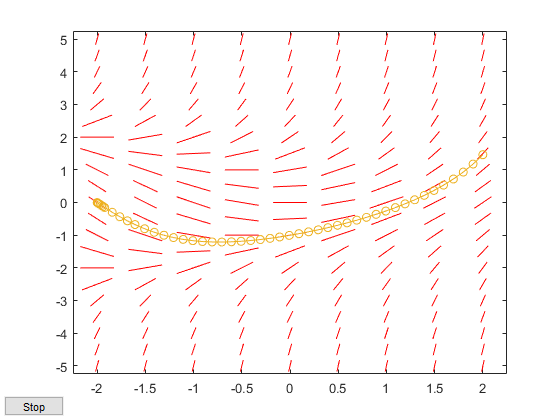
\includegraphics[width=10cm]{3slopefield}
				\caption{Slope field and solution curve of $y'=x+\frac{1}{2}y^2, y(-2)=0$}
			\end{figure}
			Examining the solution curve, we approximate $\boxed{y(2)\approx 1.5.}$
		\end{soln}

		\newpage
	\item (E\&P Problem 1.4.66) Early one morning it began to snow at a constant rate. At 7 A.M. a snowplow set off to clear a road. By 8 A.M. it had traveled 2 miles, but it took two more hours (until 10 A.M.) for the snowplow to go an additional 2 miles.
		\begin{enumerate}[(a)]
			\item Let $t=0$ when it began to snow, and let $x$ denote the distance traveled by the snowplow at time $t.$ Assuming that the snowplow clears snow from the road at a constant rate (in cubic feet per hour, say), show that
				\begin{align*}
					k\frac{dx}{dt} = \frac{1}{t}
				\end{align*}
				where $k$ is a constant.
				\begin{soln}
					Suppose snow falls at a rate $c_1$ and the plow clears snow at a rate $c_2.$ Let $s(t)$ be the amount of snow on the ground at time $t$ (suppose we are talking about the height of the snow at the untouched parts of the road). Then since the plow clears snow at a constant amount of snow, we have the relation
					\begin{align*}
						c_2 &= s(t) \frac{d}{dt} x(t) \\
						\implies \frac{dx}{dt} &= \frac{c_2}{s(t)}
					\end{align*}
					Since it snows at a constant rate, we have $s(t)=c_1t,$ and thus
					\begin{align*}
						\frac{dx}{dt} &= \frac{c_2}{c_1t} \implies \frac{c_1}{c_2}\frac{dx}{dt} = k\frac{dx}{dt} = \frac{1}{t}
					\end{align*}
				\end{soln}

			\item What time did it start snowing? (Answer: 6 A.M.)
				\begin{soln}
					The differential equation above is separable, so solving it, we have
					\begin{align*}
						k\, dx &= \frac{1}{t}\, dt \implies \int k\, dx = \int \frac{1}{t}\, dt \\
						\implies kx &= \ln t + C
					\end{align*}
					Suppose it started snowing at $T$ o'clock. Then at 7 o'clock, $t=7-T,$ and the snow plow has not moved yet. At 8 o'clock, $t=8-T,$ and the snow plow has moved 2 miles. At 10 o'clock, $t=10-T,$ and the snow plow has moved a total of 4 miles. Thus, the initial conditions are
					\begin{align*}
						x(7-T) &= 0 \\
						x(8-T) &= 2 \\
						x(10-T) &= 4
					\end{align*}
					Using these initial conditions, we have the system of equations
					\begin{align*}
						0 &= \ln (7-T) + C \\
						2k &= \ln (8-T) + C \\
						4k &= \ln(10-T) + C
					\end{align*}
					Subtracting the 1st from the 2nd, and the 2nd from the 3rd, we have
					\begin{align*}
						2k &= \ln (8-T) - \ln (7-T) = \ln \frac{8-T}{7-T} \\
						2k &= \ln (10-T) - \ln(8-T) = \ln \frac{10-T}{8-T} \\
						\implies \frac{8-T}{7-T} &= \frac{10-T}{8-T} \implies T=6
					\end{align*}
					Thus, it started snowing at \boxed{6 \text{ A.M.}}
				\end{soln}

		\end{enumerate}

		\newpage
	\item (E\&P Application 1.4) As in Eq (7) of this section, the solution of a separable differential equation reduces to the evaluation of two indefinite integrals. It is tempting to use a symbolic algebra system for this purpose. We illustrate this approach using the logistic differential equation
		\begin{align*}
			\frac{dx}{dt} = ax-bx^2 \tag{1}
		\end{align*}
		For your own personal logistic equation, take $a=m/n$ and $b=1/n$ in Eq (1), with $m$ and $n$ being the largest two distinct digits (in either order) in your student ID number.
		\begin{enumerate}[(a)]
			\item First generate a slope field for your differential equation and include a sufficient number of solution curve that you can see what happens to the population as $t\to+\infty.$ State your inference plainly.
				\begin{soln}
					For my ID number, $m=7$ and $n=6,$ so $a=7/6$ and $n=1/6.$ Thus, $\frac{dx}{dt} = \frac{7}{6}x - \frac{1}{6}x^2.$ Using the following block of MATLAB code, we generate the slope field and a couple solution curves:
					\begin{lstlisting}
					f = @(t, x) 7*x/6 - x.^2/6;
					ode45(f, [0, 10], -0.5);
					ode45(f, [3, 10], -0.5);
					ode45(f, [6, 10], -0.5);
					ode45(f, [1, 10], 0.5);
					ode45(f, [4, 10], 0.5);
					ode45(f, [7, 10], 0.5);
					ode45(f, [2, 10], 8.5);
					ode45(f, [5, 10], 8.5);
					ode45(f, [8, 10], 8.5);
					ode45(f, [0, 10], 0);
					ode45(f, [0, 10], 7);
					\end{lstlisting}
					\begin{figure}[ht]
						\centering
						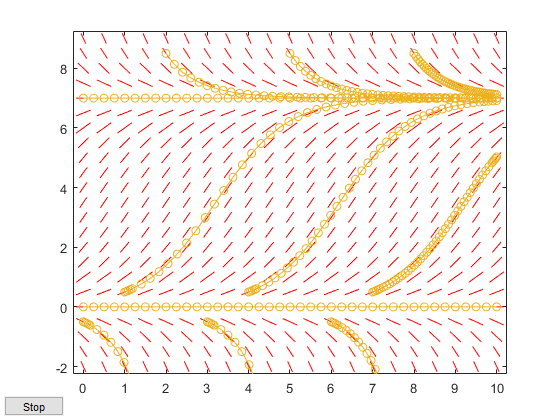
\includegraphics[width=10cm]{5aslopefield}
						\caption{Slope field and solution curves of $x'=\frac{7}{6}x-\frac{1}{6}x^2$}
					\end{figure}
					From the slope field, 0 and 7 are unstable and stable equilibrium points, respectively. As $t\to\infty,$ 
					\begin{align*}
						x(t) \to \begin{cases}
							7 & \text{ if } x_0 > 0 \\
							0 & \text{ if } x_0 = 0 \\
							-\infty & \text{ if } x_0 < 0
						\end{cases}
					\end{align*}
				\end{soln}

			\item Next use a computer algebra system to solve the differential equation symbolically; then use the symbolic solution to find the limit of $x(t)$ as $t\to+\infty.$ Was your graphically based inference correct? 
				\begin{soln}
					We could use a computer algebra system, or we could just solve this by hand since it's separable\ldots Clearly $\frac{7}{6}x-\frac{1}{6}x^2 =  \frac{1}{6}x(7-x),$ so $x=0$ and $x=7$ are critical points. Suppose $x(0)=x_0$ is the initial condition. Then
					\begin{align*}
						\frac{6}{7x-x^2}\, dx &= dt \\
						\implies \int\frac{6}{x(7-x)}\, dx &= \int dt \\
						\implies \int \frac{7}{6}\left( \frac{1}{x} + \frac{1}{7-x} \right)\, dx &= t + C \\
						\implies \frac{6}{7} \left( \ln \abs{x}-\ln\abs{7-x} \right) &= t+C \\
						\implies \ln \frac{\abs{x}}{\abs{7-x}} &= \frac{7}{6}t + C \\
						\implies \abs{\frac{x}{7-x}} &= Ce^{7t/6} \\
						\implies \abs{\frac{x_0}{7-x_0}} &= C \\
						\implies \abs{\frac{x}{7-x}} &= \abs{\frac{x_0}{7-x_0}}e^{7t/6}
					\end{align*}
					Now, we can drop the absolute value signs because for $x$ near $x_0,$ the two ratios have the same sign. If $x_0,$ then we trivially have $x(t)\equiv0.$ Otherwise, letting $K=\frac{7-x_0}{x_0},$ we can solve for $x(t)$ to get
					\begin{align*}
						x(t) = \frac{7}{1+Ke^{-7t/6}}
					\end{align*}
					Now, when $x_0>7,$ we have $-1<K<0,$ so $1+Ke^{-7t/6}<1\implies \frac{7}{1+Ke^{-7t/6}}>7.$ As $t\to\infty, e^{-7t/6}\to 0,$ so $x(t)\to 7$ from above.

					When $0<x_0<7,$ we have $K>0,$ so $1+Ke^{-7t/6}>1\implies \frac{7}{1+Ke^{-7t/6}}<7.$ Thus, $x(t)\to 7$ from below. Clearly, when $x_0=7,$ the solution is $x(t)\equiv 7.$

					When $x_0<0,$ we have $K<-1.$ Thus, as $t\to \frac{6}{7}\ln(-K),$ we have
					\begin{align*}
						1+Ke^{-7t/6}\to 1+Ke^{-\ln(-K)} = 1 + K\left( \frac{1}{-K} \right) = 0
					\end{align*}
					from below since $1+Ke^{-7t/6}<0.$ Thus, $\frac{7}{1+Ke^{-6t/7}}\to-\infty$ That is, the solution tends towards $-\infty$ as $t$ grows. These results all agree with the graphical inference.
				\end{soln}
				\newpage

			\item Finally, state and solve a numerical problem using the symbolic solution. For instance, how long does it take $x$ to grow from a selected initial value $x_0$ to a given target value $x_1?$
				\begin{soln}
					As an example, for the sake of simplicity, suppose we start at $x(0)=1=x_0$ and let $x_1=2.$ From above, we have
					\begin{align*}
						K &= \frac{7-x_0}{x_0} = \frac{7-1}{1} = 6 \\
						\implies x(t) &= \frac{7}{1+6e^{-7t/6}}
					\end{align*}
					We wish to solve for $t_1$ when $x(t_1)=2,$ so
					\begin{align*}
						x(t_1) &= \frac{7}{1+6e^{-7t_1/6}} = 2 \\
						\implies \frac{7}{2} &= 1+6e^{-7t_1/6} \\
						\implies e^{-7t_1/6} &= \frac{5}{12} \\
						\implies t_1 &= \frac{6}{7}\ln\frac{12}{5}
					\end{align*}
					Thus, at $t_1=\frac{6}{7}\ln\frac{12}{5},$ the solution will have grown from 1 to 2.
				\end{soln}

		\end{enumerate}

		\newpage
	\item Tumor Growth
		\begin{enumerate}[(a)]
			\item (E\&P Problem 2.1.30) A tumor may be regarded as a population of multiplying cells. It is found empirically that the "birth rate" of the cells in a tumor decreases exponentially with time, so that $\beta(t)=\beta_0e^{-\alpha t}$ (where $\alpha$ and $\beta_0$ are positive constants), and hence
				\begin{align*}
					\frac{dP}{dt} = \beta_0 e^{-\alpha t}P, \quad P(0)=P_0
				\end{align*}
				Solve this initial value problem for
				\begin{align*}
					P(t)=P_0\exp\left( \frac{\beta_0}{\alpha}\left( 1-e^{-\alpha t} \right) \right)
				\end{align*}
				Observe that $P(t)$ approaches the finite limiting population $P_0\exp(\beta_0/\alpha)$ as $t\to+\infty.$
				\begin{soln}
					This ODE is separable, so we have
					\begin{align*}
						\frac{1}{P}\, dP &= \beta_0 e^{-\alpha t}\, dt \\
						\implies \int \frac{1}{P}\, dP &= \int \beta_0 e^{-\alpha t}\, dt \\
						\implies \ln P &= -\frac{\beta_0}{\alpha} e^{-\alpha t} + C \\
						\implies P(t) &= \exp\left(-\frac{\beta_0}{\alpha} e^{-\alpha t} + C\right)
					\end{align*}
					Using the initial value $P(0)=P_0,$ we have 
					\begin{align*}
						P(0) = P_0 &= \exp\left( -\frac{\beta_0}{\alpha} e^{-\alpha\cdot 0} + C \right) = \exp\left( -\frac{\beta_0}{\alpha} + C \right) \\
						\implies C &= \ln P_0 + \frac{\beta_0}{\alpha}
					\end{align*}
					so the particular solution is
					\begin{align*}
						P(t) &= \exp\left( \ln P_0 + \frac{\beta_0}{\alpha} - \frac{\beta_0}{\alpha} e^{-\alpha t} \right) = P_0 \exp\left( \frac{\beta_0}{\alpha} (1-e^{-\alpha t}) \right)
					\end{align*}
					as desired. Note that as $t\to+\infty,$ the $e^{-\alpha t}$ in the numerator tends to 0, so $P(t)\to P_0 e^{\beta_0/\alpha}.$
				\end{soln}

			\item (E\&P Problem 2.1.31) For the tumor of Problem 30, suppose that at time $t=0$ there are $P_0=10^6$ cells and that $P(t)$ is then increasing at the rate of $3\times 10^5$ cells per month. After 6 months the tumor has doubled (in size and in number of cells). Solve numerically for $\alpha,$ and then find the limiting population of the tumor.
				\begin{soln}
					From the given information, we know that $\beta_0 = \frac{3\times 10^5}{10^6} = 0.3$ is the initial birth rate, and that at $t=6,$ the population has doubled so $P(6)=2P_0.$ From our solution in Problem 30,
					\begin{align*}
						P(t) &= P_0 \exp\left( \frac{\beta_0}{\alpha}(1-e^{-\alpha t}) \right) \\
						\implies P(6) &= P_0 \exp\left( \frac{0.3}{\alpha} (1-e^{-6\alpha})\right) = 2P_0 \\
						\implies 2 &= \exp\left( \frac{0.3}{\alpha}(1-e^{-6\alpha}) \right)
					\end{align*}
					Using a numerical equation solver, we find $\boxed{\alpha\approx0.3915}$ and the limiting population is
					\begin{align*}
						P_\infty &= P_0 e^{\beta_0/\alpha} = 10^6 \exp\left( \frac{0.3}{0.3915} \right) \approx \boxed{2.1518\times 10^6}
					\end{align*}
				\end{soln}

		\end{enumerate}

		\newpage
	\item (E\&P 2.2.10) First solve the equation $f(x)=0$ to find the critical points of the given autonomous differential equation $dx/dt=f(x).$ Then analyze the sign of $f(x)$ to determine whether each critical point is stable or unstable, and construct the corresponding phase diagram for the differential equation. Next, solve the differential equation explicitly for $x(t)$ in terms of $t.$ Finally, use either the exact solution or a computer-generated slope field to sketch typical solution curves for the given differential equation, and verify visually the stability of each critical point.
		\begin{align*}
			\frac{dx}{dt} = 7x-x^2-10
		\end{align*}
		\begin{soln}
			We first solve $f(x)=-x^2+7x-10 = 0$ to get the critical points of the autonomous differential equation. Factoring, $f(x)=-(x-2)(x-5)$ so the critical points are $x=2$ and $x=5.$

			Since this is a downward opening parabola, $f(x)$ is non-negative on $[2, 5]$ and negative elsewhere. Thus, according to the phase diagram below, $x=2$ is unstable, and $x=5$ is stable.
			\begin{center}
				\begin{asy}
					import graph;

					path xaxis = (-10, 0) -- (18, 0);
					Label xlabel = Label('$x$', position=EndPoint);
					draw(xaxis, arrow=Arrows, L=xlabel);

					dot( (-2, 0) );
					dot( (10, 0) );
					label('2', (-2, 0), S);
					label('5', (10, 0), S);

					draw( (-3, 0) -- (-8, 0), arrow=Arrow(TeXHead), blue+linewidth(1.5));
					draw( (-1, 0) -- (9, 0), arrow=Arrow(TeXHead), blue+linewidth(1.5));
					draw( (16, 0) -- (11, 0), arrow=Arrow(TeXHead), blue+linewidth(1.5));
				\end{asy}
			\end{center}
			The ODE is separable, so bringing separating (and a little reformatting), 
			\begin{align*}
				\frac{-1}{x^2-7x+10} \, dx &= dt 
			\end{align*}
			In order to integrate the left hand side, we must do a partial fraction decomposition. Let $A, B\in \RR.$ Then the decomposition is given by
			\begin{align*}
				\frac{-1}{(x-2)(x-5)} &= \frac{A}{x-2} + \frac{B}{x-5} = \frac{A(x-5) + B(x-2)}{(x-2)(x-5)} \\
				\implies -1 &= A(x-5) + B(x-2)
			\end{align*}
			We can solve for $A$ and $B$ by substituting $x=2$ and $x=5,$ respectively, which gives
			\begin{align*}
				-1 &= A(2-5) + B(2-2) = -3A \implies A = \frac{1}{3} \\
				-1 &= A(5-5) + B(5-2) = 3B \implies B = -\frac{1}{3}
			\end{align*}
			Thus, integrating both sides of the separated ODE, we have
			\begin{align*}
				\int \frac{-1}{x^2-7x+10}\, dx &= \int dt \\
				\implies\int\left( \frac{1}{3}\cdot \frac{1}{x-2} - \frac{1}{3}\cdot\frac{1}{x-5} \right)\, dx &= t+C \\
				\implies \frac{1}{3}\ln\abs{x-2} - \frac{1}{3}\ln\abs{x-5} &= t+C \\
				\implies \ln \abs{\frac{x-2}{x-5}} &= 3t+C \\
				\implies \frac{x-2}{x-5} &= Ce^{3t} \\
				\implies x(t) &= \boxed{\frac{3}{Ce^{3t}-1} + 5}
			\end{align*}
			Using the following block of MATLAB code, we generate the slope field and a couple solution curves:
			\begin{lstlisting}
			f = @(t, x) 7*x - x.^2 - 10;
			dirfield(f, 0:0.5:10, -1:0.5:9);
			hold on;
			ode45(f, [0, 10], 1.5);
			ode45(f, [3, 10], 1.5);
			ode45(f, [6, 10], 1.5);
			ode45(f, [1, 10], 2.5);
			ode45(f, [4, 10], 2.5);
			ode45(f, [7, 10], 2.5);
			ode45(f, [2, 10], 8.5);
			ode45(f, [5, 10], 8.5);
			ode45(f, [8, 10], 8.5);
			ode45(f, [0, 10], 2);
			ode45(f, [0, 10], 5);
			\end{lstlisting}
			\begin{figure}[ht]
				\centering
				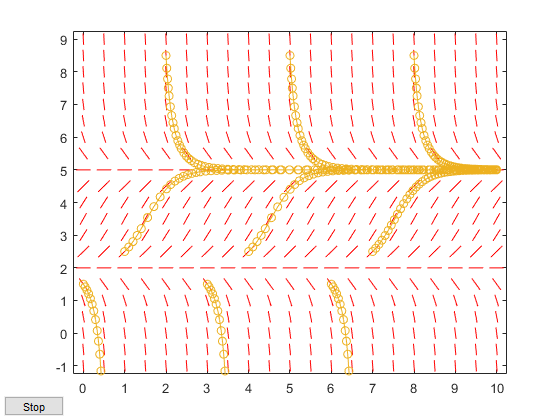
\includegraphics[width=10cm]{7slopefield}
				\caption{Slope field and solution curves of $x'=7x-x^2-10$}
			\end{figure}
			As shown by the slope field, 2 is an unstable equilibrium point, and 5 is a stable equilibrium point.
		\end{soln}

		\newpage
	\item Euler's Methods for First-Order ODEs
		\begin{enumerate}[(a)]
			\item (E\&P Problem 2.4.10) Apply Euler's method twice to approximate this solution on the interval $\left[ 0, \frac{1}{2} \right],$ first with step size $h=0.25,$ then with step size $h=0.1.$ compare the three-decimal-place values of the two approximations at $x=\frac{1}{2}$ with the value $y\left( \frac{1}{2} \right)$ of the actual solution.
				\begin{align*}
					y'=2xy^2, \quad y(0)=1; \quad y(x)=\frac{1}{1-x^2}
				\end{align*}
				\begin{soln}
					Here, $f(x, y)=2xy^2.$ Using $h=0.25,$ we have
					\begin{align*}
						y_1 &= y_0 + h\cdot f(x_0, y_0) = 1 + 0.25(2\cdot 0\cdot 1^2) = 1 \\
						y_2 &= y_1 + h\cdot f(x_1, y_1) = 1 + 0.25(2\cdot 0.25\cdot 1^2) = 1.125
					\end{align*}

					Using $h=0.1,$ we have
					\begin{align*}
						y_1 &= y_0 + h\cdot f(x_0, y_0) = 1 + 0.1(2\cdot 0\cdot 1^2) = 1 \\
						y_2 &= y_1 + h\cdot f(x_1, y_1) = 1+0.1(2\cdot 0.1\cdot 1^2)=1.02 \\
						y_3 &= y_2 + h\cdot f(x_2, y_2) = 1.02 + 0.1(2\cdot 0.2\cdot 1.02^2) = 1.062 \\
						y_4 &= y_3 + h\cdot f(x_3, y_3) = 1.062 + 0.1(2\cdot 0.3\cdot 1.062^2) = 1.129 \\
						y_5 &= y_4 + h\cdot f(x_4, y_4) = 1.129 + 0.1(2\cdot 0.4\cdot 1.129^2) = 1.231
					\end{align*}

					Using the actual solution, we have $y(0.5)=\frac{1}{1-0.5^2} \approx 1.33.$
				\end{soln}

				\newpage
			\item (E\&P Problem 2.5.10) Apply the improved Euler method to approximate this solution on the interval $[0, 0.5]$ with step size $h=0.1$ Construct a table showing four-decimal-place values of the approximate solution and actual solution at the points $x=0.1, 0.2, 0.3, 0.4, 0.5.$
				\begin{align*}
					y'=2xy^2, \quad y(0)=1; \quad y(x)=\frac{1}{1-x^2}
				\end{align*}
				\begin{soln}
					Here, $f(x, y)=2xy^2.$ Using $h=0.1,$ we have
					\begin{align*}
						k_{1, 1} &= f(x_0, y_0) = 2\cdot 0\cdot 1^2 = 0 \\
						u_1 &= y_0 + h\cdot k_{1, 1} = 1 + 0.1\cdot 0 = 1 \\
						k_{1, 2} &= f(x_1, u_1) = 2\cdot 0.1\cdot 1^2 = 0.2 \\
						y_1 &= y_0 + h\cdot \frac{1}{2}\left( k_{1, 1}+k_{1, 2} \right) = 1 + 0.1\cdot \frac{1}{2}(0+0.2) = 1.01 \\
						k_{2, 1} &= f(x_1, y_1) = 2\cdot 0.1\cdot 1.01^2 = 0.204 \\
						u_2 &= y_1 + h\cdot k_{2, 1} = 1.01 + 0.1\cdot 0.204 = 1.0304 \\
						k_{2, 2} &= f(x_2, u_2) = 2\cdot 0.2\cdot 1.0304^2 = 0.4247 \\
						y_2 &= y_1 + h\cdot \frac{1}{2}\left( k_{2, 1} + k_{2, 2} \right) = 1.01 + 0.1\cdot \frac{1}{2}\left( 0.204+0.4247 \right) = 1.0414 \\
						k_{3, 1} &= f(x_2, y_2) = 2\cdot 0.2\cdot 1.0414^2 = 0.4338 \\
						u_3 &= y_2 + h\cdot k_{3, 1} = 1.0414+0.1\cdot 0.4338 = 1.0848 \\
						k_{3, 2} &= f(x_3, u_2) = 2\cdot 0.3\cdot 1.0848^2 = 0.7061 \\
						y_3 &= y_2 + h\cdot \frac{1}{2}\left( k_{3, 1} + k_{3, 2} \right) = 1.0414 + 0.1\cdot \frac{1}{2}\left( 0.4338 + 0.7061 \right) = 1.0984 \\
						k_{4, 1} &= f(x_3, y_3) = 2\cdot 0.3\cdot 1.0984^2 = 0.7239 \\
						u_4 &= y_3 + h\cdot k_{4, 1} = 1.0984 + 0.1\cdot 0.7239 = 1.1708 \\
						k_{4, 2} &= f(x_4, u_4) = 2\cdot 0.4\cdot 1.1708^2 = 1.0966 \\
						y_4 &= y_3 + h\cdot \frac{1}{2}\left( k_{4, 1} + k_{4, 2} \right) = 1.0984 + 0.1\cdot \frac{1}{2}\left( 0.7239 + 1.0966 \right) = 1.1894 \\
						k_{5, 1} &= f(x_4, y_4) = 2\cdot 0.4\cdot 1.1894^2 = 1.1318 \\
						u_5 &= y_4 + h\cdot k_{5, 1} = 1.1894 + 0.1\cdot 1.1318 = 1.3026 \\
						k_{5, 2} &= f(x_5, u_5) = 2\cdot 0.5\cdot 1.3026^2 = 1.6967 \\
						y_5 &= y_4 + h\cdot \frac{1}{2}\left( k_{5, 1} + k_{5, 2} \right) = 1.1894 + 0.1\cdot \frac{1}{2}\left( 1.1318 + 1.6967 \right) = 1.3309
					\end{align*}
					Thus, the table of approximate and exact values at the points $0.1, 0.2, 0.3, 0.4, 0.5$ are
					\begin{center}
						\begin{tabular}{c||c|c|c|c|c}
							$x$ & 0.1 & 0.2 & 0.3 & 0.4 & 0.5 \\
							\hline
							$y_i$ & 1.01 & 1.0414 & 1.0984 & 1.1894 & 1.3309 \\
							\hline 
							$y(x)$ & 1.0101 & 1.0417 & 1.0989 & 1.1905 & 1.3333
						\end{tabular}
					\end{center}
				\end{soln}

		\end{enumerate}

\end{enumerate}

\end{document}
